\chapter{Background}
\label{chap:background}

In this chapter, topics such as citizen science, gamification, and speech corpus will be further described. Additional terms relevant to the research will also be defined and clarified, to ensure all research topics are clear. 

\section{Citizen Science}

\subsection{Origins}

The citizen science practice, although not formally defined as so, date back at least a couple of millennia. In ancient China, migratory locusts frequently destroyed harvests, and residents have helped to track outbreaks for some 2,000 years \cite{irwin2018no}. More recently, in 1890, citizen contribution was adopted by the Cooperative Weather Service \cite{quayle1991effects}, where amateurs send collected weather data to the National Weather Service, and continues to provide such data. Later in 1900, the ornithologist Frank Chapman proposed a new holiday tradition - a "Christmas Bird Census" \cite{harden1985christmas}, in which the public would count sighted birds in a predefined area. The Christmas Bird Count contributed to more than 200 publications in the scientific field \cite{kosmala2016assessing}, and the data collected assists the assessment of the health of bird populations, as well as help guide conservation action. In 1966, a similar census started by the North American Breeding Bird Survey contributed to more than 670 publications. The UK Butterfly Monitoring Scheme \cite{pollard1994monitoring}, started in 1976, assess trends in the abundance of butterflies within the United Kingdom, and have supported more than 100 publications.

\subsection{Definition}

The term "Citizen Science" was formally used by Alan Irwin, a sociologist now based at the Copenhagen Business School, with his book "Citizen science: A study of people, expertise and sustainable development" \cite{irwin1995citizen}. Irwin defined citizen science both as “science which assists the needs and concerns of citizens” and as “a form of science developed and enacted by the citizens themselves”. This term was soon modified to describe "a research technique using members of the public to gather or analyze data" \cite{bonney2009citizen}. However, with so many forms of contribution, citizen science now takes a more flexible concept, which can be adapted and applied within diverse situations and disciplines. To encompass this flexibility, the European Citizen Science Association \cite{robinson2018ten} set out some key principles which as a community they believe underlie good practice in citizen science. Appendix \ref{app:ten-principles} lists all ten principles.

\subsection{Classifications}

Below are some classifications in which citizen science projects can be divided:

\subsubsection{Volunteer Involvement}

An initial classification based on volunteer involvement \cite{follett2015analysis}: 
\begin{itemize}
    \item Contributory, where participants contribute to data collection and sometimes help analyze and disseminate results
    \item Collaborative, where citizens also analyze samples, design the study, interpret the data, draw conclusions and disseminate results
    \item Co-created, where they participate in all stages of the project, including defining questions, developing hypotheses, drawing conclusions, discussing results and answering new questions
\end{itemize}

\subsubsection{Goals of the study}

An alternative classification for these initiatives has been suggested by \cite{wiggins2011conservation}, and is based on the goals of the study:

\begin{itemize}
    \item Action projects, initiated by volunteers designed to encourage intervention in local concerns;
    \item Conservation projects, addressing natural resource management goals;
    \item Investigation projects, focusing on scientific research goals in a physical setting;
    \item Virtual projects, also focusing on scientific goals, but entirely based on information technology with all volunteer interaction occurring online;
    \item Education projects; often performed in the classroom or school grounds as part of the science curriculum.
\end{itemize}

\subsubsection{Topic of study}

An additional way of classifying citizen science projects is based on the topic of study, for example, astronomy, archaeology, and biology \cite{wiggins2011conservation}. 

\subsubsection{This work}

If these classifications are to be applied in this work, it should be categorized as a \textbf{contributory virtual speech corpus} citizen science project.

\section{Gamification}

Gamification has been a trending topic as a means of supporting user engagement, being commonly employed in the private sector but also in education, health, government, and science, taking advantage of the widespread activity of game playing \cite{kreitmair2019citizen}. The desire of gamifying services and businesses lies in bringing positive, intrinsically motivating \cite{ryan2000self}, "gamefull" experiences \cite{huotari2012defining} into a service. In the following sections, gamification is (1) defined accordingly to the literature, (2) established through motivational affordances - or game elements, (3) and characterized by some psychological and behavioral outcomes.

\subsection{Definition}

Gamification is commonly defined as "the use of elements of game design in non-game contexts" \cite{deterding2011game}. Although simple, this definition incorporates the succinct method used by gamification. An alternative interpretation by \cite{huotari2012defining} states that gamification is "a process of enhancing a service with affordances for gameful experiences in order to support user's overall value creation". The latter conceptualization suggests the interaction of two actors: (1) the user (using the service) is the creator of value while (2) the service provider can merely provide affordances for the user to experience gamefulness. Gamification can be conceptualized in three main parts \cite{hamari2014does}: 1) the implemented motivational affordances, 2) the resulting psycholgical outcomes, and 3) the further behavioral outcomes. These parts are further described below: 

\subsection{Motivational affordances (game elements)}

A literature review of empirical studies on gamification by \cite{hamari2014does} defines a list of 10 commonly motivational affordances implemented in table \ref{tab:motivational-affordances}. These 24 peer-reviewed studies were examined, indicating a large variety of different game elements added. The most commonly found were points, leaderboards and badges.

\begin{table}[h]
    \centering
    \caption{Quantity of motivational affordances implemented in 24 gamification publications}
    \begin{tabular}{|c|c|}
        \hline Motivational Affordance & Publications (out of 24) \\
        \hline Points & 9 \\
        \hline Leaderboard & 10\\ 
        \hline Achievements/Badges & 9 \\
        \hline Levels & 6 \\
        \hline Story/Theme & 6 \\
        \hline Clear goals & 4 \\
        \hline Feedback & 6 \\
        \hline Rewards & 4 \\
        \hline Progress & 4 \\
        \hline Challenge & 7 \\
        \hline
    \end{tabular}
    \caption*{Source: \cite{hamari2014does}}
    \label{tab:motivational-affordances}
\end{table}

\subsection{Psychological and behavioral outcomes}

A gamified service can have both psychological outcomes and behavioral outcomes. The former focuses on the ramifications of the contributor having "gameful" experiences. Aspects such as motivation, attitude and enjoyment. The latter generally refers to the behavior of the contributor as a result to the use of the service. Statistical analyses of contributions in a gamified environment serves as one example, aiding in concluding whether the research have had positive effects on some of the motivational affordances of the gamification implementations.

\subsection{This work}

One of the main elements of this work is the addition of gamification elements to a voice recording application, thereby laying the foundations for user engagement necessary in a citizen science application.

\subsection{Crowdsourcing}

Refers to the practice of outsourcing a task originally performed by its employees to an undefined and generally large network of people \cite{howe2006rise}. Its purpose lies in taking advantage of "wisdom of the crowd", whereby multiple people may be better at solving a given problem than a single individual, or simply to spread the workload across a large number of people, in particular, when the work does not lend itself to automation \cite{kreitmair2019citizen}. Many citizen science initiatives are by design a crowdsourcing project, utilizing the workforce of many to accomplish an objective.

\subsection{This work}

This work is also one crowdfunding citizen science project, relying in the contribution of many towards the construction of a speech corpus.

\section{Citizen Science Projects}

With the recent growth of citizen science, various breakthroughs were made possible. Below are some of the most relevant projects in the virtual space, some of which apply gamification to engage contributors.

\subsection{Foldit}

\begin{figure}[ht]
    \centering
    \caption{Foldit - Unfolded (and unstable) Streptococcal Protein Puzzle}
    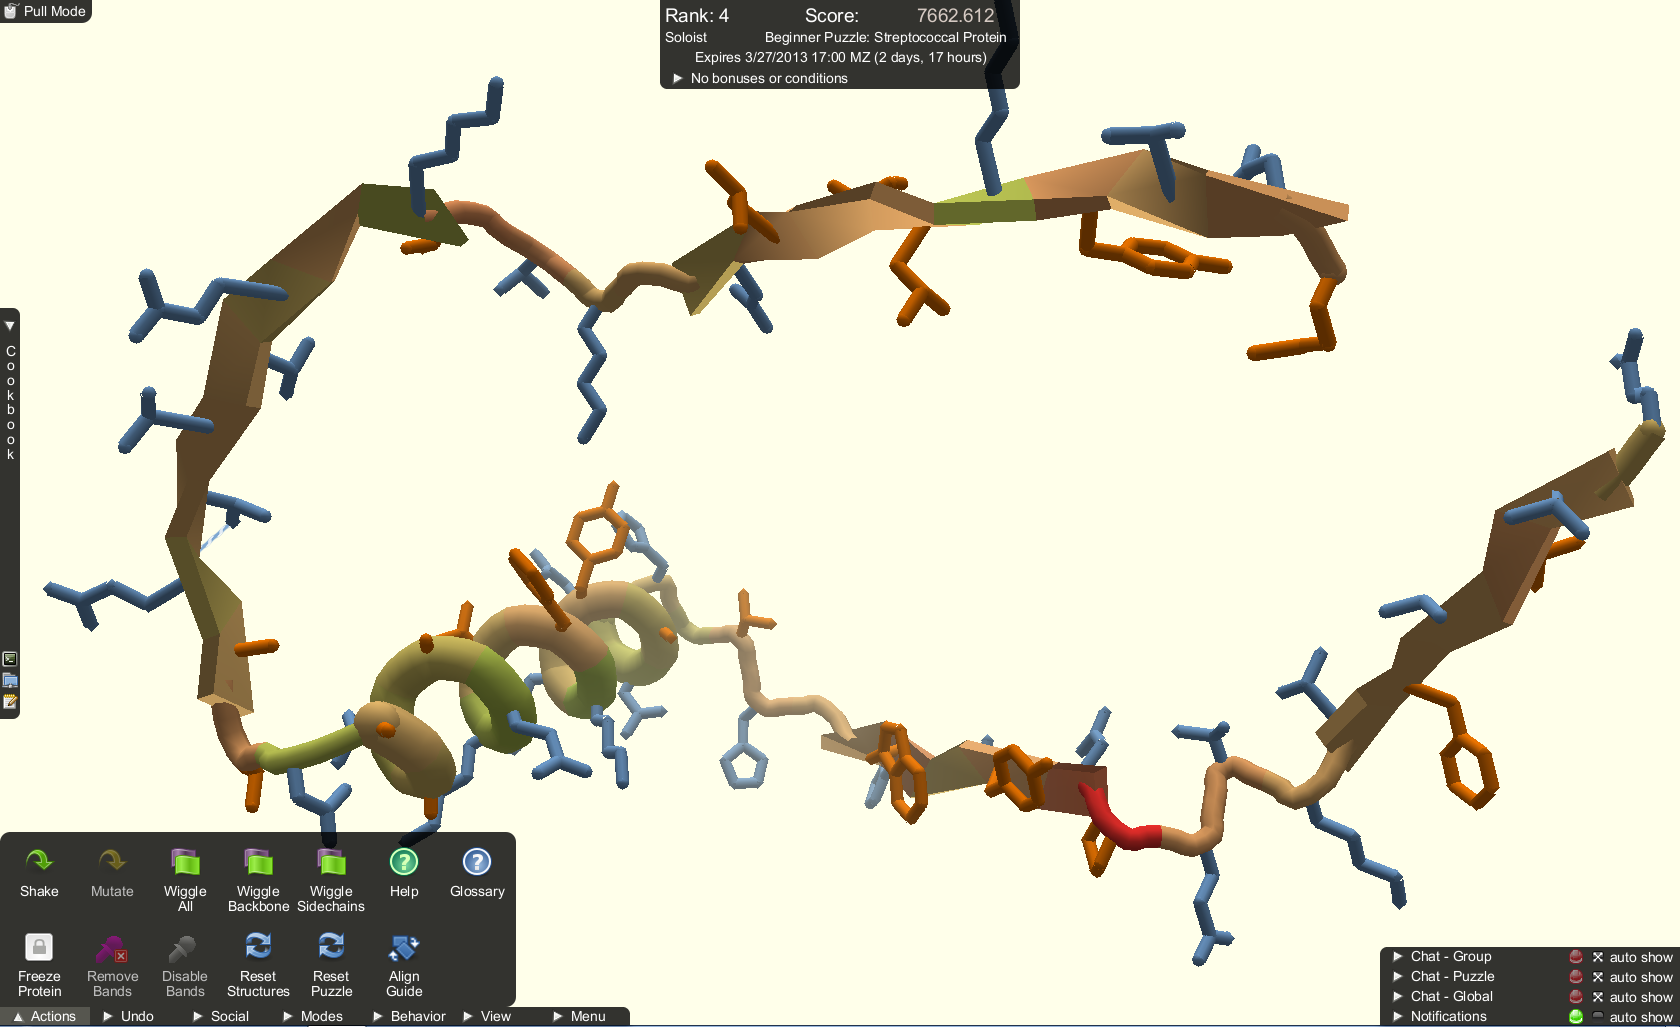
\includegraphics[width=0.8\linewidth]{images/background/foldit-problem.png}
    \caption*{Source: \cite{foldit-protein-problem}}
    \label{fig:foldit-problem}
\end{figure}

Foldit, designed by researchers at the University of Washington, is a game in which gamers solve protein folding patterns, a central challenge in biochemistry, by virtually wiggling, shaking and pulling shapes to create small stable structures, as well as developing their own algorithms for solving protein folding \cite{bourzac2008enlisting}. 

\begin{figure}[ht]
    \centering
    \caption{Foldit - Folded up Streptococcal Protein Puzzle}
    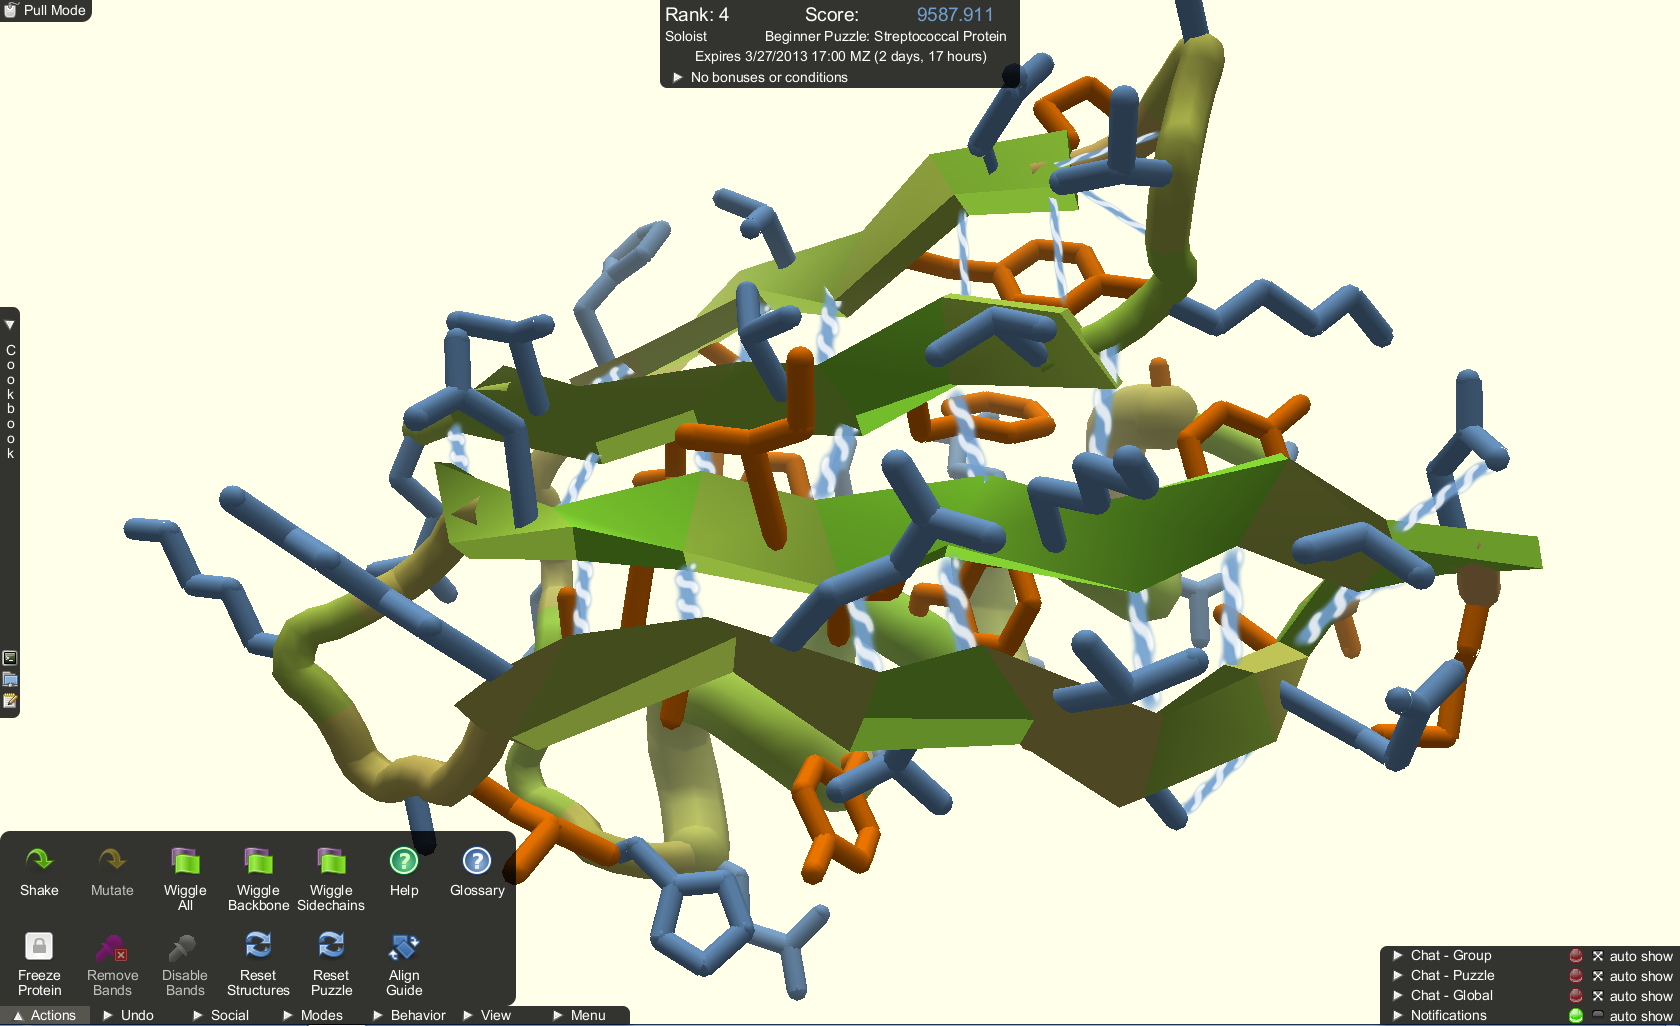
\includegraphics[width=0.8\linewidth]{images/background/foldit-solution.png}
    \caption*{Source: \cite{foldit-protein-solution}}
    \label{fig:foldit-solution}
\end{figure}

As the moment of this article, Foldit has had 20 peer-reviewed articles in a number of journals and conferences \cite{foldit2021publications}. Some relevant breakthroughs are a potential target for HIV drug development \cite{khatib2011crystal}, redesign of the catalyst for the Diels-Alder reaction \cite{eiben2012increased}, and improvement of cryo-electron microscopy atomic model building and refinement \cite{khatib2019building}.

\subsubsection{Gamification in Foldit}

To appeal to the general public, Foldit applies gamification in many different elements. The main objective of the game is to obtain the most stable and folded protein. To encourage this optimization, the user interface assigns a score to the protein, relative to how well it is folded. The best solutions to these puzzles are displayed in a ranking system, to promote competition between users. Another element to aid engagement is social. Users create and join groups, and members of groups can share puzzle solutions. These groups have been found to be useful in training new players.

\subsection{EyeWire}

\begin{figure}[ht]
    \centering
    \caption{EyeWire game interface}
    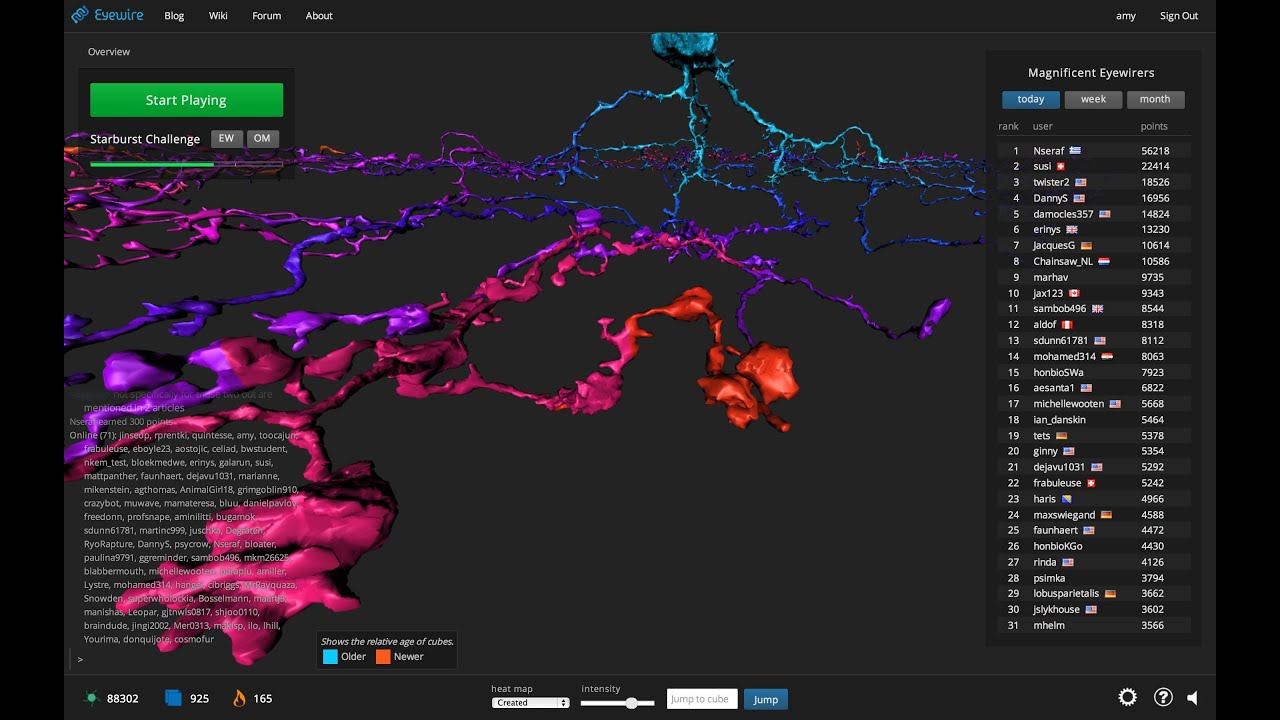
\includegraphics[width=0.8\linewidth]{images/background/eyewire.jpg}
    \caption*{Source: \cite{eyewire2014how}}
    \label{fig:eyewire-game-interface}
\end{figure}

EyeWire is a Web-based citizen science game that aims to create a detailed atlas of the human brain. Nonprofessionals are asked to map connections of neurons which reside in the back of the human eye. This mapping is done through 3D-transformed functional magnetic resonance images (fMRI), and combines crowd contributions with machine learning algorithms to help neuroscientists to achieve a better understanding of visual stimuli processing by humans.

\subsubsection{Gamification in EyeWire}

EyeWire transforms the complex task of brain mapping into smaller (micro) tasks via a gaming interface with several elements associated \cite{seaborn2015gamification}. This has been identified as a positive motivation for a player's participation \cite{tinati2016because}. Other elements such as music, sound effects, interactive tutorials, leaderboard, and a chat interface add to the overall experience, creating a fun experience. According to a survey on EyeWire motivation \cite{tinati2016because}, 57\% out of 349 respondents considered the the game entertaining.

\subsection{Galaxy Zoo}

\begin{figure}[ht]
    \centering
    \caption{Hubble's Galaxy Classification Schema to help new players classify galaxies}
    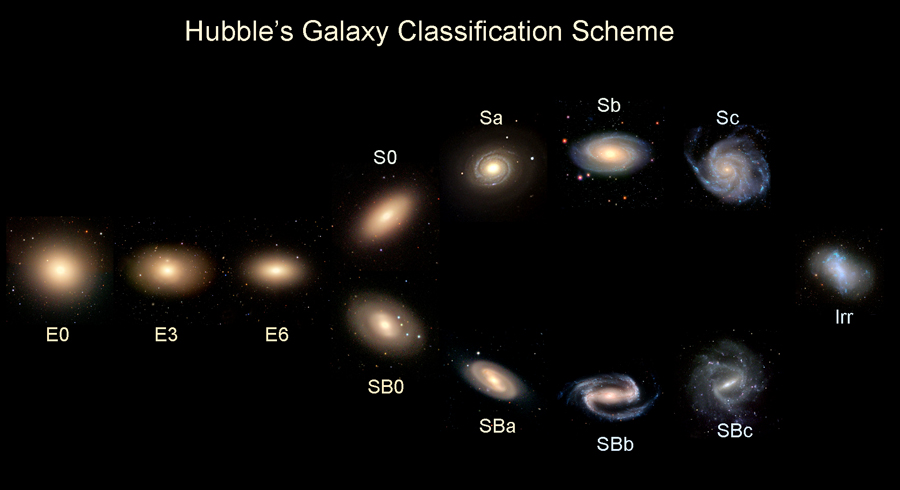
\includegraphics[width=0.8\linewidth]{images/background/galaxyzoo-training.jpg}
    \caption*{Source: \cite{galaxyzoo2010hubble}}
    \label{fig:galaxyzoo-hubble}
\end{figure}

In July 2007, Galaxy Zoo was a simple online citizen science initiative that asked volunteers to morphologically classify selected images of galaxies by the Sloan Digital Sky Survey (\cite{york2000sloan} executed at Apache Point Observatory by the SDSS 2.5m telescope). In this first iteration, Galaxy Zoo has had more than 100,000 volunteers classifying nearly 900,000 galaxies \cite{lintott2011galaxy}. The unexpected popularity has inspired the creation of Zooniverse, hosting project using the same technique across many research areas \cite{zooniverse2021galaxy}.

After its end in 2009, Galaxy Zoo was followed by Galaxy Zoo 2 (GZ2). The second incarnation extends the original Galaxy Zoo classifications for a subset of the brightest galaxies in the legacy release, measuring more detailed morphological features. This iteration contributed to 60 million classifications on more than 250,00 SDSS galaxies by more than 80,000 volunteers \cite{galaxyzoo22021volunteers}.

Including the latest issue of Galaxy Zoo (started in 2018), the initiative has supported the publication of 82 articles \cite{galaxyzoo2021publications}, helping analyze elements such as: galaxy rotation, color of elliptical galaxies, galaxy dust, galaxy bulges, etc.

\subsubsection{Gamification in Galaxy Zoo}

Galaxy Zoo utilizes the Zooniverse platform for data classification (illustrated in figure \ref{fig:zooniverse-platform}). This platform is not a gamified environment, thus relying on other forms of engagement to retain users, such as interest in astronomy, enjoyment of looking at galaxy pictures, desire and excitement to contribute to scientific research, etc \cite{raddick2009galaxy}.

\subsection{Zooniverse}

\begin{figure}[h]
    \centering
    \caption{Zooniverse Platform, connecting volunteers with scientists}
    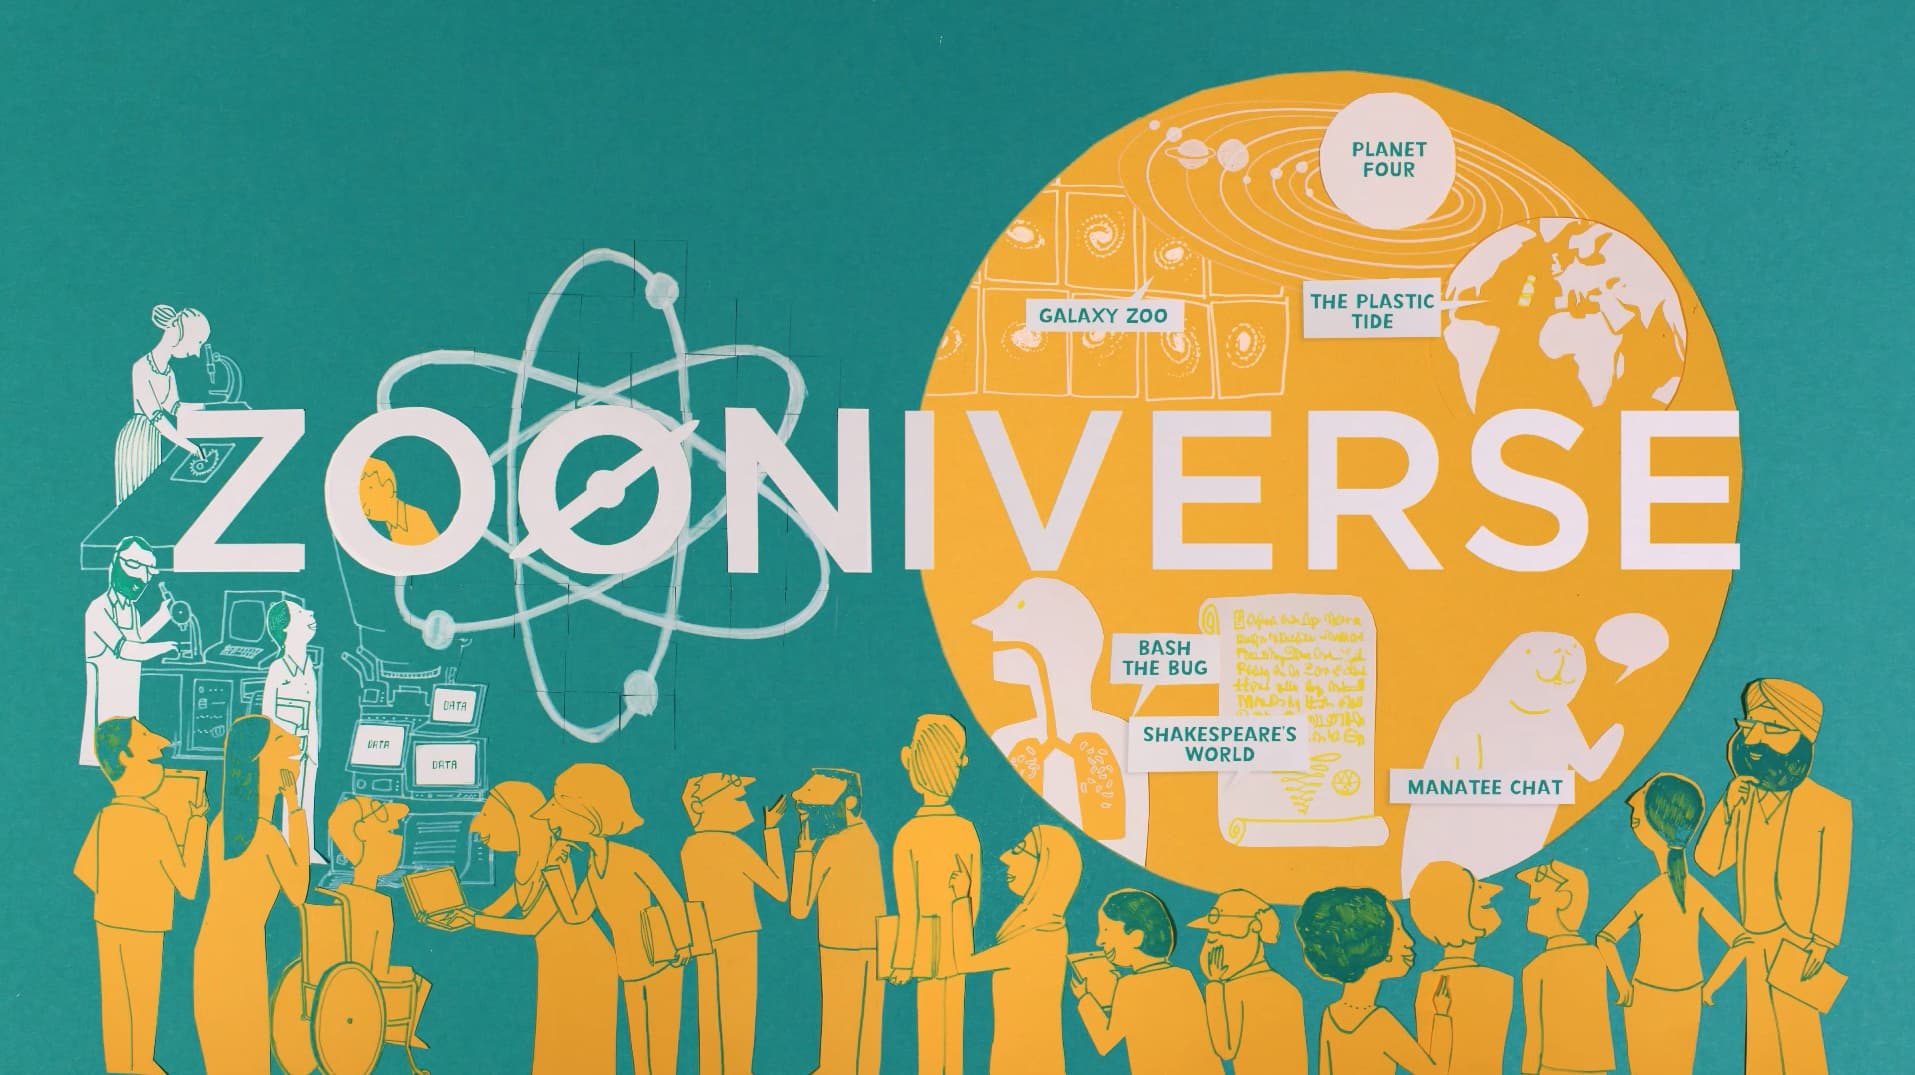
\includegraphics[width=0.7\linewidth]{images/background/zooniverse.jpg}
    \caption*{Source: \cite{zooniverse-logo}}
    \label{fig:zooniverse-platform}
\end{figure}

Zooniverse is a platform for citizen science projects. It connects more than a million volunteers around the world to assist professional researchers. The platform has a simple interface for input and classification of data, as well as the creation and management of projects.

This collaborative platform has enabled over 300 of scientific publications, with publications on the discovery and classification of stars, planets, supernovas; humanities, animal identification, classification of whale calls, datasets, etc. The following projects started in Zooniverse and each have their own characteristics:

\subsection{Penguin Watch}

\begin{figure}[ht]
    \centering
    \caption{Penguin Watch interface - Penguins are marked as adults and chicks}
    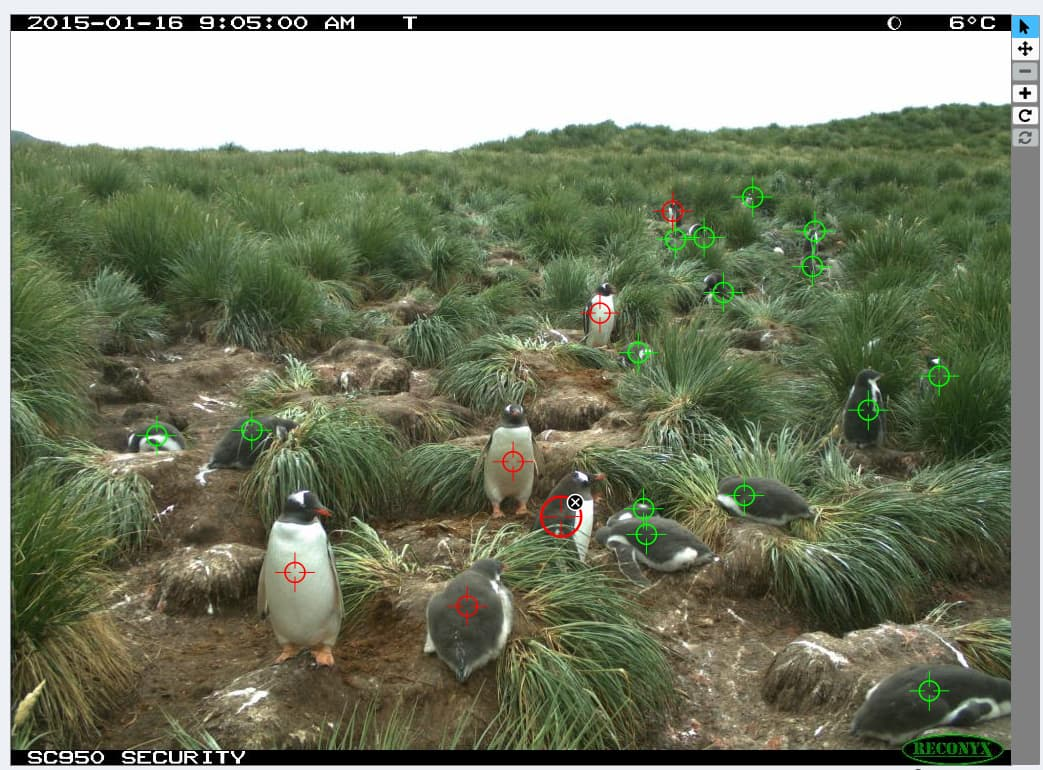
\includegraphics[width=0.8\linewidth]{images/background/penguinwatch.jpg}
    \caption*{Source: \cite{penguin2015watch}}
    \label{fig:penguin-watch}
\end{figure}

The Penguin Watch citizen science project states that by monitoring the population change in seabirds like penguins, it is possible to identify changes occurring in the wider ecosystem. These changes can help create health indicators of the marine environment, but the lack of the ability to collect and analyze such amounts of data made a team of researchers create the Penguin Watch initiative. Contributors help identify penguins in images of various sites over the world by using a web interface in Zooniverse, with its interface depicted in figure \ref{fig:penguin-watch}.

\subsubsection{Gamification in Penguin Watch}

Like with GalaxyZoo, Penguin Watch runs their contribution platform over Zooniverse. While the platform does take responsibility for maintaining infrastructure and service management, it does not include gamification elements in the classification interface.

\subsection{Aggregated Contributions}

The table \ref{tab:cs-contributions} contains an aggregated list of contributors and contributions from the projects described above.

\begin{table}[h]
\centering
\caption{Contribution for online citizen science projects mentioned above}
\label{tab:cs-contributions}
\begin{threeparttable}
    \small{
    \begin{tabular}{|c|c|c|}
        \hline 
        Project & Contributors & Publications \\ \hline
        Foldit & 855,350 \cite{foldit2021players} & 20 \cite{foldit2021publications} \\ \hline
        EyeWire & 300,000 \cite{eyewire2017players} & 3 \cite{eyewire2021publications} \\ \hline
        Penguin Watch & 28,500 \cite{penguin2021players} & 10 \cite{penguin2021publications} \\ \hline
        Galaxy Zoo (2007-2009) & 100,000+ \cite{lintott2011galaxy} & \multirow{3}{*}{82 \cite{galaxyzoo2021publications}\tnote{~a}} \\ \cline{1-2} 
        Galaxy Zoo 2 (2009-2013) & 80,000+ \cite{galaxyzoo22021volunteers} & \\ \cline{1-2} 
        Galaxy Zoo (2018-2021) & 61,149 \cite{galaxyzoo2021players} & \\ \hline 
    \end{tabular}}
    \begin{tablenotes}
        \item[a] Across all Galaxy Zoo Iterations, including Radio and Supernova Galaxy Zoo.
    \end{tablenotes}
\end{threeparttable}
\caption*{Source: Author}
\end{table}

\section{Natural Language Processing}

The field of natural language processing encompasses a variety of topics, which involves the computational processing and understanding of human language \cite{otter2020survey}. Formats in which this understanding can occur include (but are not limited to) sentiment analysis, sentence prediction, text translation, text-to-speech conversion, and speech recognition \cite{chowdhury2003natural}. Natural language processing is based on both a set of theories and a set of technologies. Its foundations lie in a number of disciplines, namely, computer and information sciences, linguistics, mathematics, electrical and electronic engineering, artificial intelligence and robotics, and psychology \cite{chowdhury2003natural}. Three key disciplines to the practice are: Linguistics - focusing on formal, structural models of language and the discovery of language universals - in fact, the field of NLP was originally referred to as Computational Linguistics; Computer Science - concerning itself with developing interal representations of data and efficient processing of these structures and; Cognitive Psychology - looking at language as a window into human cognitive process, and has the goal of modeling the use of language in a psychologically plausible way  \cite{liddy2001natural}.

Nonetheless, to use the aforementioned applications (such as text translations, and speech recognition), it is necessary to analyze and decipher the core fundamentals of language understanding \cite{otter2020survey}. These core fundamentals come in many forms, such as (1) language modeling, which emphasyzes the associations among naturally occurring words \cite{DBLP:journals/corr/cs-CL-0108005}; morphological processing, dealing with decomposition of words and identification of relevant parts of speech; syntactic processing, or parsing, which builds sentence diagrams to understand the structure of phrases \cite{woolf2010building}; and semantic processing, which attempts to distill meaning of words, phrases and higher level components in text \cite{otter2020survey}.

With more research and advancement in technology, many of the core fundamentals have been studied, allowing for more practical applications surging within a mobile environment \cite{yu2016automatic}, with virtual assistants such as Alexa, Siri, and Google Now; language translation now suffers minor changes in meaning across languages \cite{de2018no}, offered by companies such as Google, IBM, and Microsoft.

\subsection{Automatic Speech Recognition}

Automatic Speech recognition is aimed to enable natural human-machine translation and has been an intensive research area for decades \cite{yu2016automatic}. Enhancements and optimizations of core technologies such as Gaussian mixture models (GMMs), hidden Markov models (HMMs), mel-frequency cepstral coeffients (MFCCs), n-gram language models (LMs), discriminative training and various adaptation techniques have been developed, mostly prior the new millennium. These core fundamentals, akin to the ones in natural language processing, greatly advance the state of the art in the related fields.

Yet, in the past several years, there has been a surge of interest in automatic speech recognition \cite{jurafsky2016speech}. This change was led by its increased demands on mobile devices, with new speech applications such as voice search, short message dictation and virtual speech assistants. The means to achieve these demands have also been developed, with (1) more computing power available \cite{ECONOMOU2004279}, (2) advanced deep learning techniques \cite{graves2013speech}. However, these tools emphasize on the ever-growing need for data.

\section{Speech Corpus}

In the context of automatic speech recognition, data to enable the training and testing of a ASR system is called a speech corpus. They are voice datasets, that curate a collection of audio recordings of a spoken language. Data labeling is one feature they may have, characterizing additional text files with transcriptions of the words spoken, sometimes even aligning the texts with the time they are spoken in the recording. Figure \ref{fig:annotated-speech-corpus} shows a annotated utterance for speech corpus for the Euronounce project \cite{demenko2009applying}.

\begin{figure}[h]
    \centering
    \caption{Example of annotated utterance from the German-Polish speech corpus of the Euronounce project.}
    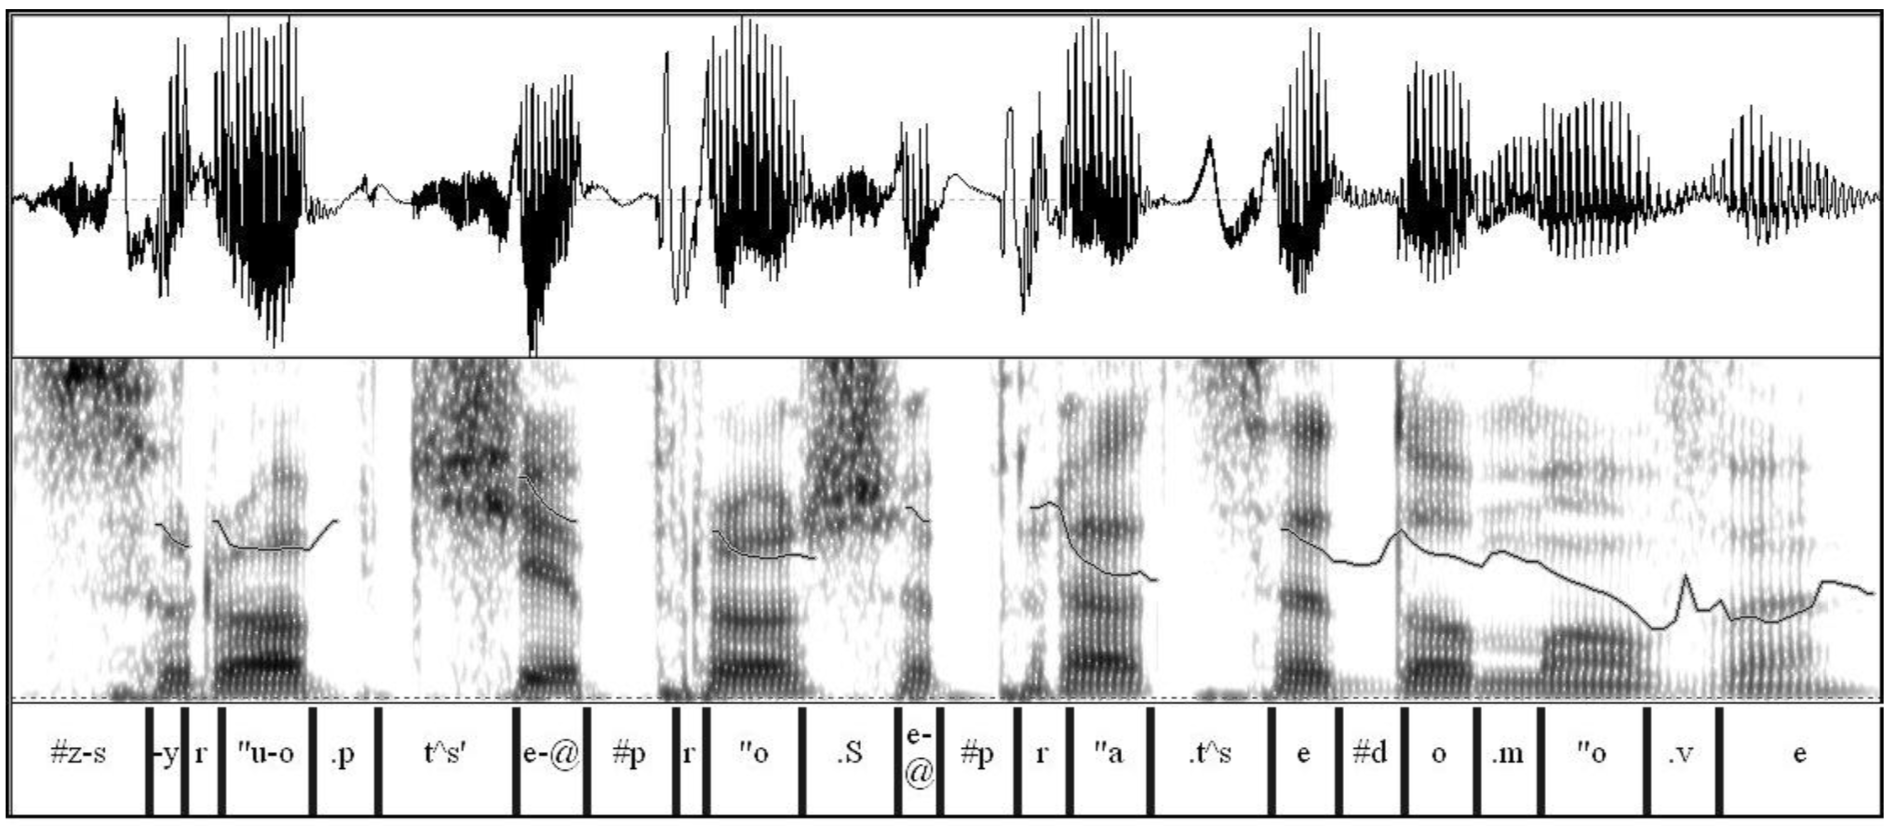
\includegraphics[width=0.8\linewidth]{images/background/annotated-speech-corpus.png}
    \caption*{Source: \cite{demenko2009applying}}
    \label{fig:annotated-speech-corpus}
\end{figure}

Another feature to aid in speech recognition is speaker metadata. 

...

\subsubsection{This work}

This section outlines the overall characteristics of the main objective of this work: the construction and validation of a speech corpus.

\section{Noisy data}

A common issue with these croudsourced online datasets lies in data quality. Disparities in recorded noise, environment change, recording length variation, and general quality of the recording are intrinsically associated with these contributions, since volunteers have each their own devices and recording conditions. To mitigate these issues, work has been made in the post-processing of these recordings \cite{krishna2019speech}.

\section{Licencing}

\subsection{GPL}

\subsection{CC0}
